\begin{center}
 \vspace{-3cm}
    \huge{6}
    \noindent\makebox[\linewidth]{\rule{\paperwidth}{0.4pt}}
    \small
    \small{А\,Н\,Д\,Р\,Е\,Й Н\,И\,К\,О\,Л\,А\,Е\,В\,И\,Ч К\,О\,Л\,М\,О\,Г\,О\,Р\,О\,В}
\end{center}
\vspace{1cm}

\begin{minipage}{0.45\textwidth}
  определения которых есть множество М = \{A, B\} из букв А и В и значения которых принадлежат тому же множеству, т. е. отображения множества М в себя.
  
 \parindent=0.5cm Таких функций существует всего четыре. Зададим их табличным способом:
\begin{center}
\begin{tabular}{|p{0.9cm}|c|c|c|c|}
\hline
     $x$ & $f_1(x)$ & $f_2(x)$ & $f_3(x)$ & $f_4(x)$ \\ \hline
     A & A & B & A & B \\ \hline
     B & A & B & B & A \\
\hline
\end{tabular}
\end{center}

 \parindent=0.5cm Функци $f_1$ и $f_2$  являются {\it константами} т. е. {\it постоянными}: множество значений каждой из этих функций состоит их одного-единственного элемента.
 
 \parindent=0.5cm Функции $f_3$ и $f_4$ отображают множество М на себя. Функция $f_3$ может быть задана формулой 
\begin{center}
$f_3(x) = x.$
\end{center}

 \parindent=0.5cm Это - {\it тождественное} отображение: каждый элемент множества Е отображается в самого себя.
 
 \parindent=0.5cm Чтобы закончить выясление смысла самого понятия «функция», остается обратить внимание на то, что выбор букв для обозначения «независимого переменного», т.е. произвольного элемента области определения, и «зависимого переменного», т.е. произвольного элемента множества значений, совершенно несуществен. Записи
\begin{center}
$x \xrightarrow{f} \sqrt{x},$   $\xi \xrightarrow{f} \sqrt{\xi},$ $y \rightarrow{} \sqrt{y},$ \\
\bigskip
$f(x) = y = \sqrt{x},$ $f(\xi) = \eta = \sqrt{\xi},$ $f(y) = x = \sqrt{y}$
\end{center}
определяют {\it одну и ту же функцию $f$}, которая отображает неотрицательное число в арифметический квадратный корень из него. Пользуясь любой из этих записей, мы получим $f(1)=1, f(4)=2, f(9)=3$ и т.д.
\begin{center}
    
\normalsize{{\bf Обратимая функция}}
\end{center}
\parindent=0.5cm Функция
\begin{center}
$y=f(x)$
\end{center}
называется {\it обратимой}\footnote[$^2$]{$^2${\it Происхождение названия выясняются дальше: функция обратима, если для нее существует обратная ей функция.}}, если каждое свое

\end{minipage}
\hfill
\begin{minipage}{0.45\textwidth}
  значение она принимает один-единственный раз. Таковы функции $f_3(x)$ и $f_4(x)$ из примера 4. Функции же $f_1(x)$ и $f_2(x)$ из примера 4 и функции из примеров 1, 2, и 3 {\it необратимы}.
  
 \parindent=0.5cm Чтобы доказать, что какая-либо функция необратима, достаточно указать какие-либо два значения аргумента $x_1 \neq x_2$ , для которых
  \begin{center}
  $f(x_1) = f(x_2)$
  \end{center}
 
 \parindent=0.5cm В примере 3 достаточно заметить, что Петя дежурит как 1-го, так и 5-го февраля. Поэтому функция примера 3 необратима.
 
 \parindent=0.5cm {\bf Пример 5.} Функция 
  \begin{center}
  $x \xrightarrow{f} y = - \sqrt{x}$ 
  \end{center}
  обратима. Она определена на множестве {\bf R$_+$} неотрицательных чисел. Множеством ее значений является множество 
  \begin{center}
  {\bf R$_-$}=$(-\infty;0]$
  \end{center}
  всех неположительных чисел. Задав любое $y$ из множества {\bf R$_-$}, можно найти соотвествующее $x$ по формуле $x = y^2$ .
  
 \parindent=0.5cm  Функция $g$ 
  \begin{center}
  $ y \xrightarrow{g} x = y^2$ при $ y \leq 0,$ 
  \end{center}
  есть функция, {\it обратная} к функции $f$. Она отображает множество {\bf R$_-$} на множество {\bf R$_+$}. Как уже говорилось, выбор букв для обозначения независимого и зависимого переменного несуществен.
  
 \parindent=0.5cm  Функции $f$и $g$ можно записать в виде 
  \begin{center}
  $f(x) = -\sqrt{x}$ при $x \geq 0$,\\
  \bigskip
  $g(x) = x^2$ при $x \leq 0. $
  \end{center}
  
  \parindent=0.5cm На рисунке 4 изображены графики взаимно обратных функций $f$ и $g$. 
  
 \parindent=0.5cm  {\bf Пример 6.} Функция $f$, заданная таблицей
  \begin{center}
  \begin{tabular} {|c|c|c|c|c|c|}
  \hline
  $x$ & А & Б & В & Г & Д \\ \hline
  $y$ & 3 & 1 & 2 & 5 & 4 \\ \hline
  \end{tabular}
  \end{center}
  определена на множестве первых пяти букв русского алфавита, а на множество ее значений есть множество первых пяти натуральных чи-
\end{minipage}

\thispagestyle{empty}
\newpage
\begin{center}
    \huge{7}
    \noindent\makebox[\linewidth]{\rule{\paperwidth}{0.4pt}}
    \small {Ч\,Т\,О Т\,А\,К\,О\,Е Ф\,У\,Н\,К\,Ц\,И\,Я\,?}
\end{center}
\vspace{1cm}
\begin{minipage}{0.45\textwidth}
сел. Обратная функция $g$ задается таблицей
\begin{center}
\begin{tabular}{|c|c|c|c|c|c|}
\hline
$x$ & 1 & 2 & 3 & 4 & 5 \\ \hline
$y = g(x)$ & Б & В & А & Д & Г\\\hline
\end{tabular}
\end{center}

\parindent=0.5cm На рисунке 5 даны графики этих функций.

\parindent=0.5cm Дадим точные определения. Пусть $f$ - отображение множества Е на множество М. Если для любого элемента $y$ из множества М существует один-единственный элемент
\begin{center}
$x = g(y)$
\end{center}
\end{minipage}
\hfill
\begin{minipage}{0.45\textwidth}

\begin{center}
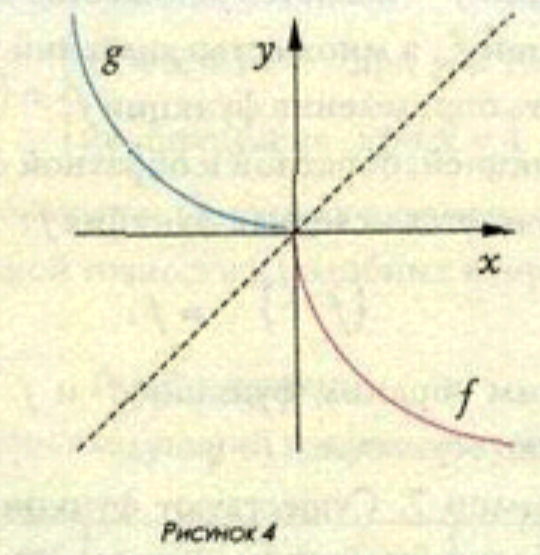
\includegraphics[width=5cm]{pic.png}\\
\end{center}

\end{minipage}
\thispagestyle{empty}
 
